\title{[Lab6] Let's Play GANs!}
\author{0616014 楊政道}
\maketitle
\thispagestyle{fancy}
\section{Introduction}
\subsection{實驗目的}
\paragraph{}
本次實驗目的為使用生成對抗網路(Generative Adversarial Networks, 簡稱GAN), 來完成給定條件下的圖片生成。欲生成的圖片由8種顏色和3種形狀的物體, 最多3個所陳列在某個全灰背景下的圖片。
\begin{figure}[!ht]
    \begin{center} 
        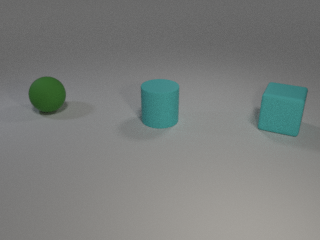
\includegraphics[width=5cm]{dataset_ex.png}
        \caption{訓練資料範例}
    \end{center} 
\end{figure}
\section{Implementation details}
\subsection{DataLoader}
\paragraph{}
由於這次的資料是圖片, 為了避免讀取圖片佔用到太多的計算資源倒置GPU使用率太低, 因此先對圖片預先存成torch tensor的二進制檔案, 並且預先做好圖片的轉換(Resize, ToTensor和Normalize)。
\begin{lstlisting}[language=Python]
class Dataset(Dataset):

    def __init__(self, path):
        self.labels = torch.load('dataset/labels.pth').long()
        self.images = torch.load('dataset/images.pth')

    def __getitem__(self, index):
        images, labels = [], []
        for i in range(3):
            images.append(self.images[index * 3 + i])
            labels.append(self.labels[index * 3 + i])
        images = torch.stack(images)
        labels = torch.stack(labels)
        return images, labels

    def __len__(self):
        return self.labels.size(0) // 3
\end{lstlisting}
\subsection{Task}
\paragraph{}
原本的問題是給一個不固定長度的陣列, 輸出一張有陣列中的物體的圖。考量到不固定長度訓練起來有難度, 因此將原本的問題改成, 給一張圖和一個要加上去的物體, 輸出原本的圖加上該物體的RNN問題。
\begin{figure}[!ht]
    \begin{center} 
        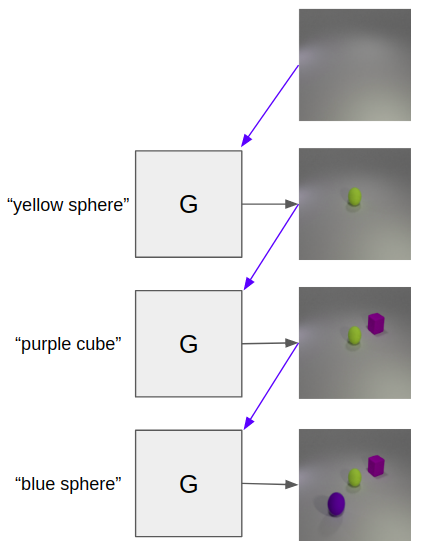
\includegraphics[width=5cm]{task.png}
        \caption{Task}
    \end{center} 
\end{figure}
\subsection{GAN}
\paragraph{}
GAN的整體架構就是Discriminator, Generator, 還有一個RNN, RNN的作用在於處理收到的condition sequence, RNN輸出的output則用於GAN的condition, hidden則繼續傳下去等待下一個input。
\begin{figure}[!ht]
    \begin{center} 
        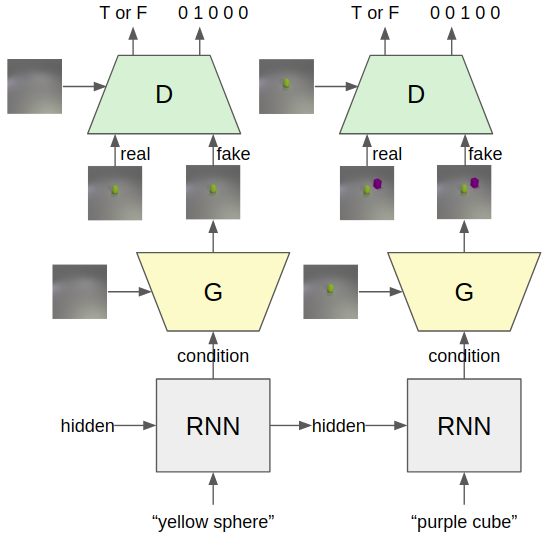
\includegraphics[width=5cm]{gan.png}
        \caption{GAN 架構}
    \end{center} 
\end{figure}
\newpage
\subsection{Discriminator}
\paragraph{}
Discriminator目的要分辨輸入的圖為真還是假, 並且分辨上面的物件類別。輸入為上一張圖跟目標圖, 各做三次的DownConv後相減, 可以獲得兩張圖差異的feature map, 後面再根據這個差異來判斷圖的真假以及要加上去的物件的類別。
\begin{figure}[!ht]
    \begin{center} 
        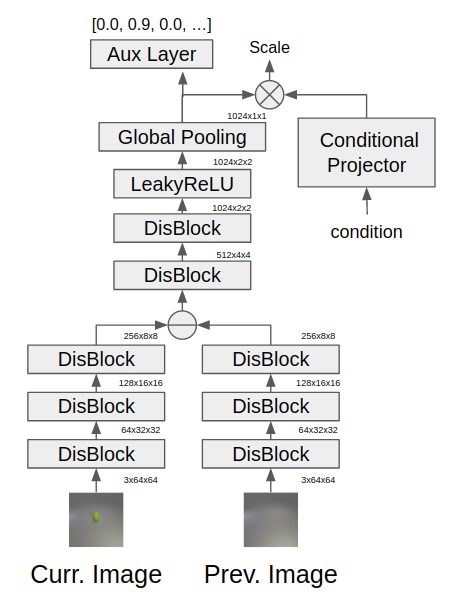
\includegraphics[width=5cm]{dis.png}
        \caption{Discriminator 架構}
    \end{center} 
\end{figure}
\paragraph{}
DisBlock參考ResNet的架構, 經過一層DisBlock解析度都會/2。
\paragraph{}
Loss function有4個, 分別為d\_real, d\_fake, aux\_loss, gradient\_penalty。
$$Loss = - d\_real + d\_fake + aux\_loss + gradient\_penalty$$
\paragraph{}
使用到了Conditional Projector, WGAN-GP, spectral\_norm。
\newpage
\subsection{Generator}
\paragraph{}
Generator目的要根據condition來生出對應的圖片。輸入為一個noise和一個conditional vector,中間層時接上prev\_image,輸出一個3x64x64的圖片。
\begin{figure}[!ht]
    \begin{center} 
        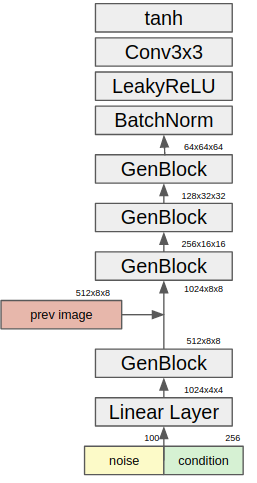
\includegraphics[width=5cm]{gen.png}
        \caption{Generator 架構}
    \end{center} 
\end{figure}
\paragraph{}
Loss function只有一項, 要讓生出來的圖被discriminator辨認為真。
$$Loss = -d\_fake $$
\section{Discussion}
\subsection{GAN學習不穩}
\paragraph{}
原始的GAN學習上非常不穩, 同樣的參數跑不同次結果會有很大的不同。原因為當Discriminator學習太過快速讓Generator沒辦法跟上時, 對於Generator來說的gradient太小, 所以會訓練失敗。解決的方法為弱化Discriminator。
\subsection{Discriminator後的Sigmoid Layer}
\paragraph{}
Sigmoid會讓遠離0兩端的gradient太小, 導致gradient desent有困難, 將sigmoid層拔掉之後輸出一個scale, 可以解決此問題。
\subsection{gradient penalty}
\paragraph{}
由於discriminator的sigmoid layer被拔掉了, 為了避免discriminator沒有下限的往下學習,因此需要加上regurization項來穩定discriminator的學習。下面為gradient penalty的實作code。
\begin{lstlisting}[language=Python]
    def __gradient_penalty(self, d_real, real_images):
        batch_size = d_real.size(0)
        grad = autograd.grad(
            outputs = d_real.sum(),
            inputs = real_images,
            create_graph=True,
            retain_graph=True,
            only_inputs=True
        )[0]
        return (grad ** 2).view(batch_size, -1).sum(1)
\end{lstlisting}
\subsection{Hyper parameters}
Discriminator的optimzer為Adam(lr=4e-4, betas=(0, 0.9)), Generator的optimizer為Adam(lr=1e-4, betas=(0, 0.9)), RNN的optimizer為Adam(lr=1e-3), 訓練140epoches。
\section{Result}
\paragraph{}
如下為test.json的結果
\begin{figure}[!ht]
    \begin{center} 
        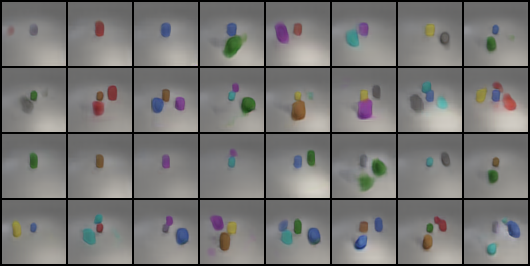
\includegraphics[width=10cm]{result1.png}
        \caption{test.json的結果, accuracy=0.89}
    \end{center} 
\end{figure}
\paragraph{}
隨意生一筆測資的結果
\begin{figure}[!ht]
    \begin{center} 
        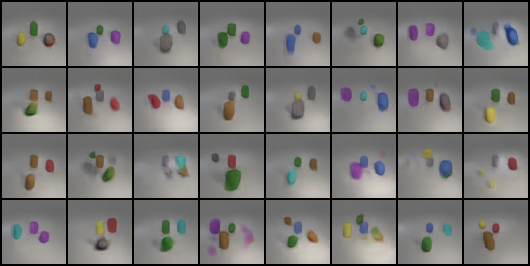
\includegraphics[width=10cm]{result2.png}
        \caption{custom.json的結果, accuracy=0.83}
    \end{center} 
\end{figure}
\section{Appendix}
\subsection{Generator Structure}
\begin{lstlisting}
(gen): GenNet(
    (c_proj): Linear(in_features=256, out_features=256, bias=True)
    (l0): Linear(in_features=356, out_features=16384, bias=True)
    (block1): GenBlock(
      (ac): LeakyReLU(negative_slope=0.01)
      (upsample): Upsample(scale_factor=2.0, mode=nearest)
      (cbn1): ConditionalBatchNorm2d(
        (bn): BatchNorm2d(1024, eps=1e-05, momentum=0.1, affine=False, track_running_stats=True)
        (fc): Linear(in_features=256, out_features=2048, bias=True)
      )
      (cbn2): ConditionalBatchNorm2d(
        (bn): BatchNorm2d(512, eps=1e-05, momentum=0.1, affine=False, track_running_stats=True)
        (fc): Linear(in_features=256, out_features=1024, bias=True)
      )
      (c0): Conv2d(1024, 512, kernel_size=(1, 1), stride=(1, 1))
      (c1): Conv2d(1024, 512, kernel_size=(3, 3), stride=(1, 1), padding=(1, 1))
      (c2): Conv2d(512, 512, kernel_size=(3, 3), stride=(1, 1), padding=(1, 1))
    )
    (block2): GenBlock(
      (ac): LeakyReLU(negative_slope=0.01)
      (upsample): Upsample(scale_factor=2.0, mode=nearest)
      (cbn1): ConditionalBatchNorm2d(
        (bn): BatchNorm2d(1024, eps=1e-05, momentum=0.1, affine=False, track_running_stats=True)
        (fc): Linear(in_features=256, out_features=2048, bias=True)
      )
      (cbn2): ConditionalBatchNorm2d(
        (bn): BatchNorm2d(256, eps=1e-05, momentum=0.1, affine=False, track_running_stats=True)
        (fc): Linear(in_features=256, out_features=512, bias=True)
      )
      (c0): Conv2d(1024, 256, kernel_size=(1, 1), stride=(1, 1))
      (c1): Conv2d(1024, 256, kernel_size=(3, 3), stride=(1, 1), padding=(1, 1))
      (c2): Conv2d(256, 256, kernel_size=(3, 3), stride=(1, 1), padding=(1, 1))
    )
    (block3): GenBlock(
      (ac): LeakyReLU(negative_slope=0.01)
      (upsample): Upsample(scale_factor=2.0, mode=nearest)
      (cbn1): ConditionalBatchNorm2d(
        (bn): BatchNorm2d(256, eps=1e-05, momentum=0.1, affine=False, track_running_stats=True)
        (fc): Linear(in_features=256, out_features=512, bias=True)
      )
      (cbn2): ConditionalBatchNorm2d(
        (bn): BatchNorm2d(128, eps=1e-05, momentum=0.1, affine=False, track_running_stats=True)
        (fc): Linear(in_features=256, out_features=256, bias=True)
      )
      (c0): Conv2d(256, 128, kernel_size=(1, 1), stride=(1, 1))
      (c1): Conv2d(256, 128, kernel_size=(3, 3), stride=(1, 1), padding=(1, 1))
      (c2): Conv2d(128, 128, kernel_size=(3, 3), stride=(1, 1), padding=(1, 1))
    )
    (block4): GenBlock(
      (ac): LeakyReLU(negative_slope=0.01)
      (upsample): Upsample(scale_factor=2.0, mode=nearest)
      (cbn1): ConditionalBatchNorm2d(
        (bn): BatchNorm2d(128, eps=1e-05, momentum=0.1, affine=False, track_running_stats=True)
        (fc): Linear(in_features=256, out_features=256, bias=True)
      )
      (cbn2): ConditionalBatchNorm2d(
        (bn): BatchNorm2d(64, eps=1e-05, momentum=0.1, affine=False, track_running_stats=True)
        (fc): Linear(in_features=256, out_features=128, bias=True)
      )
      (c0): Conv2d(128, 64, kernel_size=(1, 1), stride=(1, 1))
      (c1): Conv2d(128, 64, kernel_size=(3, 3), stride=(1, 1), padding=(1, 1))
      (c2): Conv2d(64, 64, kernel_size=(3, 3), stride=(1, 1), padding=(1, 1))
    )
    (bn): BatchNorm2d(64, eps=1e-05, momentum=0.1, affine=True, track_running_stats=True)
    (ac): LeakyReLU(negative_slope=0.01)
    (conv): Conv2d(64, 3, kernel_size=(3, 3), stride=(1, 1), padding=(1, 1))
    (tanh): Tanh()
  )
\end{lstlisting}
\subsection{Discriminator Structure}
\begin{lstlisting}
(dis): DisNet(
    (ac): LeakyReLU(negative_slope=0.01)
    (block1): DisBlock(
      (c0): Conv2d(3, 64, kernel_size=(1, 1), stride=(1, 1))
      (c1): Conv2d(3, 64, kernel_size=(3, 3), stride=(1, 1), padding=(1, 1))
      (c2): Conv2d(64, 64, kernel_size=(3, 3), stride=(1, 1), padding=(1, 1))
      (ac): LeakyReLU(negative_slope=0.01)
      (downsample): AvgPool2d(kernel_size=2, stride=2, padding=0)
    )
    (block2): DisBlock(
      (c0): Conv2d(64, 128, kernel_size=(1, 1), stride=(1, 1))
      (c1): Conv2d(64, 128, kernel_size=(3, 3), stride=(1, 1), padding=(1, 1))
      (c2): Conv2d(128, 128, kernel_size=(3, 3), stride=(1, 1), padding=(1, 1))
      (ac): LeakyReLU(negative_slope=0.01)
      (downsample): AvgPool2d(kernel_size=2, stride=2, padding=0)
    )
    (block3): DisBlock(
      (c0): Conv2d(128, 256, kernel_size=(1, 1), stride=(1, 1))
      (c1): Conv2d(128, 256, kernel_size=(3, 3), stride=(1, 1), padding=(1, 1))
      (c2): Conv2d(256, 256, kernel_size=(3, 3), stride=(1, 1), padding=(1, 1))
      (ac): LeakyReLU(negative_slope=0.01)
      (downsample): AvgPool2d(kernel_size=2, stride=2, padding=0)
    )
    (block4): DisBlock(
      (c0): Conv2d(256, 512, kernel_size=(1, 1), stride=(1, 1))
      (c1): Conv2d(256, 512, kernel_size=(3, 3), stride=(1, 1), padding=(1, 1))
      (c2): Conv2d(512, 512, kernel_size=(3, 3), stride=(1, 1), padding=(1, 1))
      (ac): LeakyReLU(negative_slope=0.01)
      (downsample): AvgPool2d(kernel_size=2, stride=2, padding=0)
    )
    (block5): DisBlock(
      (c0): Conv2d(512, 1024, kernel_size=(1, 1), stride=(1, 1))
      (c1): Conv2d(512, 1024, kernel_size=(3, 3), stride=(1, 1), padding=(1, 1))
      (c2): Conv2d(1024, 1024, kernel_size=(3, 3), stride=(1, 1), padding=(1, 1))
      (ac): LeakyReLU(negative_slope=0.01)
      (downsample): AvgPool2d(kernel_size=2, stride=2, padding=0)
    )
    (l6): Linear(in_features=1024, out_features=1, bias=True)
    (condition_projector): Sequential(
      (0): Linear(in_features=256, out_features=1024, bias=True)
      (1): ReLU()
      (2): Linear(in_features=1024, out_features=1024, bias=True)
    )
    (aux_objective): Sequential(
      (0): Linear(in_features=1024, out_features=256, bias=True)
      (1): ReLU()
      (2): Linear(in_features=256, out_features=24, bias=True)
    )
  )
\end{lstlisting}
